%% This is based on the leaflet.tex file present in the texlive-leaflet module
%% 
%% Copyright 2014 Ankur Sinha for the Fedora Marketing Team - marketing@lists.fedoraproject.org
% Please e-mail the marketing team if you have any questions with this document

\def\filename{fedora-flyer-users.tex}
\documentclass[
%%notumble,
%%nofoldmark,
%%dvipdfm,
%%portrait,
%%titlepage,
%%nocombine,
%%a3paper,
%%debug,
%%nospecialtricks,
%%draft,
10pt
]{leaflet}


%\renewcommand*\foldmarkrule{.3mm}
%\renewcommand*\foldmarklength{5mm}

\usepackage[T1]{fontenc}
\usepackage{textcomp}
% Use this to change the paper format
\usepackage{fancyhdr}
\usepackage{graphicx}

%%\usepackage[default]{cantarell} %% Use option ``defaultsans'' to use cantarell as sans serif only
%%\usepackage[default]{comfortaa} %% looks better
%%\usepackage[T1]{fontenc}

%% helvetica
%\usepackage{helvet}
%\renewcommand*{\familydefault}{\sfdefault}
% opensans
\usepackage[default,osfigures,scale=0.95]{opensans} %% Alternatively

\usepackage[dvipsnames,usenames]{color}
\definecolor{FedoraBlue}{cmyk}{1,0.46,0,0}
\definecolor{ResolutionBlue}{cmyk}{0.573,.462,0,0.541}
\definecolor{LIGHTGRAY}{gray}{.9}
\usepackage[colorlinks=true,urlcolor=FedoraBlue]{hyperref}

%%\setlength\footskip{2cm}

\newcommand*\defaultmarker{\textsuperscript\textasteriskcentered}

%%\title{Fedora workstation}
\title{
\includegraphics[keepaspectratio,width=0.8\textwidth]{Logo_fedoralogo.png}\vspace{1cm}\\\LARGE{\textcolor{ResolutionBlue}{21\\\vspace{0.2cm}for home users}}}
\date{\Large{\textcolor{FedoraBlue}{\href{http://fedoraproject.org}{http://fedoraproject.org}}}}
\author{\href{mailto:users@lists.fedoraproject.org}{users@lists.fedoraproject.org}}

\CutLine*{1}% Dotted line without scissors
%%\CutLine{6}%  Dotted line with scissors
\CutLine*{6}%  Dotted line with scissors

%\AddToBackground{5}{%  Background of a small page
%  \put(0,0){\textcolor{Cerulean}{\rule{\paperwidth}{\paperheight}}}}

\AddToBackground*{2}{% Background of a large page
  \put(\LenToUnit{.5\paperwidth},\LenToUnit{.5\paperheight}){%
    \makebox(0,0)[c]{%
      \resizebox{.9\paperwidth}{!}{\rotatebox{35.26}{%
        \textsf{\textbf{\textcolor{LIGHTGRAY}{DRAFT}}}}}}}}

\begin{document}

\maketitle
\thispagestyle{empty}
\vspace{5cm}
\begin{center}\small{Fedora and the Infinity Logo are\\registered trademarks of Red Hat, Inc.}\end{center}

\newpage

\section{\textcolor{FedoraBlue}{Find everything easily with the Gnome overview search}}
With the new Gnome overview search, you can easily find everything you'd need - applications, documents, pictures, music, notes, software, weather forecasts, bookmarks and more!

\section{\textcolor{FedoraBlue}{All your accounts are now in one place and integrated to your applications}}
The new Gnome online accounts makes it a breeze to set up your internet accounts. GMail, Facebook, Flickr, OwnCloud, Microsoft Exchange and Windows Live are all supported along with a host of others can all be set up in one place. All your applications - Evolution, Empathy, Documents, Music, Photos are integrated to seamlessly bring your data to you.
\section{\textcolor{FedoraBlue}{Ease of installation}}
\begin{figure}[h]
  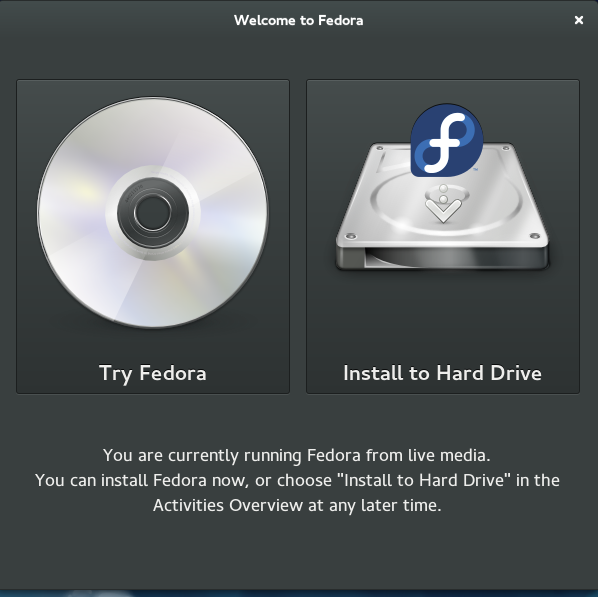
\includegraphics[keepaspectratio,width=\textwidth]{Workstation-anaconda-0-cropped.png}
\end{figure}
We want the installation of the Fedora Workstation to be as straightforward and simple as possible. In Fedora Workstation we've distilled this process down to selecting the layout of your physical media, and then pressing ``Install.'' (In fact, you can even let the installer choose the disk layout for you.) And because the future of installations is not optical disks, we ship with an easy to use tool to help you create bootable USB sticks -- just download a new Live image, right-click, and write to USB.


\section{\textcolor{FedoraBlue}{Easy access to all your software}}
\begin{figure}[h]
  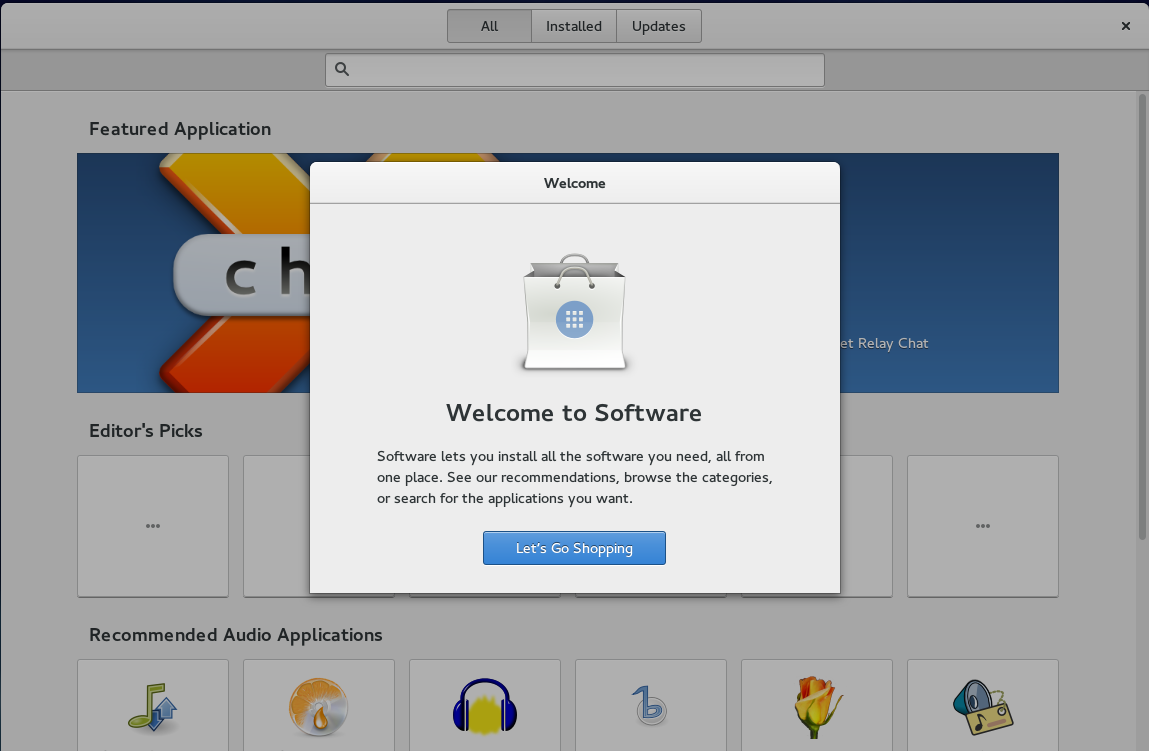
\includegraphics[keepaspectratio,width=\textwidth]{Gnome_software_welcome-cropped.png}
\end{figure}
The cornerstone of the Fedora Workstation is the Software installer, which lets you find all kinds of applications quickly and easily. The improvements to the Software installer in Fedora 21 provide a responsive and fast user experience. In addition, Fedora packagers have worked with developers around the world to greatly improve the number of featured applications.

\section{\textcolor{FedoraBlue}{Web service integration}}
We recognize you have work to do, and you want to use the tools that let you get it done. That's why we're working to make all your applications in Fedora Workstation look and feel the same. With the ability to run HTML5 web services in a chromeless window, we aim to make your apps feel like a natural extension to your desktop. More integration upgrades are coming in future Fedora Workstation releases.
\section{\textcolor{FedoraBlue}{Support for high resolution displays (HiDPI)}}
Technology never stands still. So we've spent a lot of time and effort on supporting the new generation of HiDPI displays found on new hardware like many new ultrabook models, or the Apple Retina display.

\section{\textcolor{FedoraBlue}{Tools for developers}}
We want developers to have a great experience on Fedora too! We've added various tools to help you quickly get started with your new project! Some of these are:

\subsection{\textcolor{FedoraBlue}{Improvements to the terminal application}}
The terminal has seen various enhancements to make your work even easier. Support for transparent backgrounds, automatic title updates, and the ability to search for Terminals by name in the GNOME desktop overview are some of the enhancements. 

\subsection{\textcolor{FedoraBlue}{DevAssistant}}
We recognize developers need an easy and straightforward way to set up many different programming environments. In Fedora Workstation, we offer the DevAssistant developer helper, which takes care of this setup for a large number of language runtimes and IDEs.

\section{\textcolor{FedoraBlue}{Multiple flavours}}
This Fedora Workstation release is not the only flavour of Fedora that you can use. Many other great flavours are also available:
\begin{itemize}
  \item KDE
  \item XFCE
  \item MATE
  \item LXDE
  \item Fedora Design spin
  \item Fedora Games spin
  \item \ldots and much more
\end{itemize}

Install Fedora 21 now!
\newpage

\begin{center}
  {\color{FedoraBlue}
  \LARGE{Fedora Project\vspace{1cm}}
  \Large{\href{http://fedoraproject.org}{http://fedoraproject.org}}
}
\end{center}

\section{\textcolor{FedoraBlue}{Getting Support}}
\subsection{Fedora project wiki and mailing lists}
\href{https://fedoraproject.org/wiki/Communicate}{https://fedoraproject.org/wiki/Communicate}

\subsection{Official Documentation}
\href{http://docs.fedoraproject.org}{http://docs.fedoraproject.org}

\subsection{IRC Channel}
\href{http://webchat.freenode.net/?channels=#fedora}{\#fedora @ irc.freenode.net}

\subsection{Community forums}
\href{http://ask.fedoraproject.org}{http://ask.fedoraproject.org}
\href{http://fedoraforum.org}{http://fedoraforum.org}


\section{\textcolor{FedoraBlue}{Looking to join the Fedora community?}}
Are you interested in contributing to Fedora? There are many ways you can become active in the project.  Whether you are a People Person, Designer, OS Developer, Packager or Administrator - we have a place for you. Just head to the following page and get started today!

\begin{center}\href{http://join.fedoraproject.org}{http://join.fedoraproject.org}\end{center}


\end{document}
